% !TEX TS-program = XeLaTeX
% use the following command: 
% all document files must be coded in UTF-8
\documentclass{textolivre}
% for anonymous submission
%\documentclass[anonymous]{textolivre}
% to create HTML use 
%\documentclass{textolivre-html}
% HTML compile using make4ht
% $ make4ht -c textolivre-html.cfg -u -x article "fn-in,svg,pic-align"   
%
% See more information on the repository: https://github.com/leolca/textolivre

% Metadata
\begin{filecontents*}[overwrite]{article.xmpdata}
    \Title{Scientific production of flipped learning and flipped classroom in Web of Science}
    \Author{Jesús López-Belmonte \sep Antonio-José Moreno-Guerrero \sep Juan-Antonio López-Núñez \sep Santiago Pozo-Sánchez}
    \Language{en}
    \Keywords{Bibliometric study \sep Flipped learning \sep Flipped classroom \sep Analysis of co-words \sep Web of Science database}
    \Journaltitle{Texto Livre}
    \Journalnumber{1983-3652}
    \Volume{14}
    \Issue{1}
    \Firstpage{1}
    \Lastpage{16}
    \Doi{10.35699/1983-3652.2021.26266}

    \setRGBcolorprofile{sRGB_IEC61966-2-1_black_scaled.icc}
            {sRGB_IEC61966-2-1_black_scaled}
            {sRGB IEC61966 v2.1 with black scaling}
            {http://www.color.org}
\end{filecontents*}

% used to create dummy text for the template file
\definecolor{dark-gray}{gray}{0.35} % color used to display dummy texts
\usepackage{lipsum}
\SetLipsumParListSurrounders{\colorlet{oldcolor}{.}\color{dark-gray}}{\color{oldcolor}}

% used here only to provide the XeLaTeX and BibTeX logos
\usepackage{hologo}

% used in this example to provide source code environment
%\crefname{lstlisting}{lista}{listas}
%\Crefname{lstlisting}{Lista}{Listas}
%\usepackage{listings}
%\renewcommand\lstlistingname{Lista}
%\lstset{language=bash,
        breaklines=true,
        basicstyle=\linespread{1}\small\ttfamily,
        numbers=none,xleftmargin=0.5cm,
        frame=none,
        framexleftmargin=0.5em,
        framexrightmargin=0.5em,
        showstringspaces=false,
        upquote=true,
        commentstyle=\color{gray},
        literate=%
           {á}{{\'a}}1 {é}{{\'e}}1 {í}{{\'i}}1 {ó}{{\'o}}1 {ú}{{\'u}}1 
           {à}{{\`a}}1 {è}{{\`e}}1 {ì}{{\`i}}1 {ò}{{\`o}}1 {ù}{{\`u}}1
           {ã}{{\~a}}1 {ẽ}{{\~e}}1 {ĩ}{{\~i}}1 {õ}{{\~o}}1 {ũ}{{\~u}}1
           {â}{{\^a}}1 {ê}{{\^e}}1 {î}{{\^i}}1 {ô}{{\^o}}1 {û}{{\^u}}1
           {ä}{{\"a}}1 {ë}{{\"e}}1 {ï}{{\"i}}1 {ö}{{\"o}}1 {ü}{{\"u}}1
           {Á}{{\'A}}1 {É}{{\'E}}1 {Í}{{\'I}}1 {Ó}{{\'O}}1 {Ú}{{\'U}}1
           {À}{{\`A}}1 {È}{{\`E}}1 {Ì}{{\`I}}1 {Ò}{{\`O}}1 {Ù}{{\`U}}1
           {Ã}{{\~A}}1 {Ẽ}{{\~E}}1 {Ũ}{{\~u}}1 {Õ}{{\~O}}1 {Ũ}{{\~U}}1
           {Â}{{\^A}}1 {Ê}{{\^E}}1 {Î}{{\^I}}1 {Ô}{{\^O}}1 {Û}{{\^U}}1
           {Ä}{{\"A}}1 {Ë}{{\"E}}1 {Ï}{{\"I}}1 {Ö}{{\"O}}1 {Ü}{{\"U}}1
           {ç}{{\c{c}}}1 {Ç}{{\c{C}}}1
}


\journalname{Texto Livre: Linguagem e Tecnologia}
\thevolume{14}
\thenumber{1}
\theyear{2021}
\receiveddate{\DTMdisplaydate{2020}{11}{15}{-1}} % YYYY MM DD
\accepteddate{\DTMdisplaydate{2021}{1}{7}{-1}}
\publisheddate{\DTMdisplaydate{2021}{3}{12}{-1}}
% Corresponding author
\corrauthor{Santiago Pozo-Sánchez}
% DOI
\articledoi{10.35699/1983-3652.2021.26266}
% list of available sesscions in the journal: articles, dossier, reports, essays, reviews, interviews, editorial
\articlesessionname{Educação e Tecnologia}
% Abbreviated author list for the running footer
\runningauthor{López-Belmonte et al.}
\editorname{Daniervelin Pereira}

\title{Scientific production of flipped learning and flipped classroom in Web of Science}
\othertitle{Produção científica de aprendizagem invertida e sala de aula invertida em Web of Science}
% if there is a third language title, add here:
%\othertitle{Artikelvorlage zur Einreichung beim Texto Livre Journal}

\author[1]{Jesús López-Belmonte\orcid{0000-0003-0823-3370}\thanks{Email: \url{jesuslopez@ugr.es}}}
\author[1]{Antonio-José Moreno-Guerrero\orcid{0000-0003-3191-2048} \thanks{Email: \url{ajmoreno@ugr.es}}}
\author[1]{Juan-Antonio López-Núñez\orcid{0000-0001-9881-9169}\thanks{Email: \url{juanlope@ugr.es}}}
\author[1]{Santiago Pozo-Sánchez\orcid{0000-0001-8125-4990}\thanks{Email: \url{santiagopozosanchez@gmail.com}}}

\affil[1]{Universidad de Granada, Granada, España.}

\addbibresource{article.bib}
% use biber instead of bibtex
% $ biber tl-article-template

% set language of the article
\setdefaultlanguage[variant=british]{english}
\setdefaultlanguage{spanish}
\setotherlanguage[variant=brazilian]{portuguese}

% for spanish, use:
%\setdefaultlanguage{spanish}
%\gappto\captionsspanish{\renewcommand{\tablename}{Tabla}} % use 'Tabla' instead of 'Cuadro'

% for languages that use special fonts, you must provide the typeface that will be used
% \setotherlanguage{arabic}
% \newfontfamily\arabicfont[Script=Arabic]{Amiri}
% \newfontfamily\arabicfontsf[Script=Arabic]{Amiri}
% \newfontfamily\arabicfonttt[Script=Arabic]{Amiri}
%
% in the article, to add arabic text use: \textlang{arabic}{ ... }

\usepackage{tabularx}
\usepackage{multirow}
\usepackage[defaultlines=5,all]{nowidow}

\begin{document}
\maketitle

\begin{polyabstract}
\begin{english}
\begin{abstract}
This study focuses on knowing the scientific production of the terms flipped learning and flipped classroom in specialized literature, determining their conceptual evolution, the most relevant topics and the most prolific authors. A bibliometric study has been carried out supported by a structural and dynamic analysis of co-words. Both terms have been analyzed in the Web of Science, reporting 2968 documents and observing a much higher production in the flipped classroom. Despite the fact that both terminologies are frequently used as synonyms, in the scientific community they are differentiated, observing different trends and fields of study according to the concept. The results may promote the search for a terminological consensus that clearly delimits the area covered by each concept.

\keywords{Bibliometric study \sep Flipped learning \sep Flipped classroom \sep Analysis of co-words \sep Web of Science database}
\end{abstract}
\end{english}

\begin{portuguese}
\begin{abstract}
O objetivo deste estudo é conhecer a produção científica dos termos \textit{flipped learning} e \textit{flipped classroom} na literatura especializada, determinando sua evolução conceitual, os temas mais relevantes e os autores mais prolíficos. Foi realizado um estudo bibliométrico apoiado por uma análise estrutural e dinâmica de co-palavras. Ambos os termos foram analisados na Web of Science, relatando 2.968 documentos e observando uma produção muito maior na sala de aula invertida. Apesar de ambas as terminologias serem frequentemente utilizadas como sinônimos, na comunidade científica elas se diferenciam, observando diferentes tendências e campos de estudo de acordo com o conceito. Os resultados podem promover a busca por um consenso terminológico que delimite claramente a área de abrangência de cada conceito.

\keywords{Estudo bibliométrico \sep Aprendizagem invertida \sep Sala de aula invertida \sep Análise de co-palavras \sep Banco de dados da Web of Science}
\end{abstract}
\end{portuguese}

\begin{spanish}
\begin{abstract}
El objetivo de este estudio es conocer la producción científica de los términos aprendizaje invertido y aula invertida en la literatura especializada, determinando su evolución conceptual, los temas más relevantes y los autores más prolíficos. Se realizó un estudio bibliométrico apoyado en un análisis estructural y dinámico de co-palabras. Ambos términos fueron analizados en la Web of Science, reportando 2.968 documentos y observando una producción mucho mayor en el aula invertida. Aunque ambas terminologías se utilizan a menudo indistintamente, en la comunidad científica se diferencian, observando diferentes tendencias y campos de estudio según el concepto. Los resultados pueden promover la búsqueda de un consenso terminológico que delimite claramente el alcance de cada concepto.

\keywords{Estudio bibliométrico \sep Aprendizaje invertido \sep Aula invertida \sep Análisis de co-palavras \sep Base de datos de Web of Science.}
\end{abstract}
\end{spanish}

% if there is another abstract, insert it here using the same scheme
\end{polyabstract}


\section{Introduction}\label{sec-intro}
The present work deals with the state of the question in the scientific literature of one of the didactic approaches that are booming in the field of education: the emerging methodology known as flipped learning or flipped classroom \cite{cabi2018,chen_findings_2019,zainuddin_how_2019}. Due to its dual denomination, this study emerges to explore in the different scientific works about the state, development, as well as the similarities and differences between both terms. The relevance of this research is based on the novelty of this study in the impact literature. With the completion of this literary analysis, the gap between the conceptual level and the generation of new knowledge about the state of the matter have been closed since no work has been reported to date to achieve the aforementioned purposes. 

This innovative learning model has been implemented in the field of education for almost a decade. Its origin dates back to 2011, when its predecessors –Jonathan Bergmann and Aaron Sams– carried out a teaching praxis through audiovisual materials hosted on the Internet, so that students with regular attendance problems could view it and –consequently– follow the same learning rhythm as the rest of peers \cite{bergmann_flip_2012}. 

At present, education is positioned as one of the most promising approaches in the technopedagogical field \cite{hinojo_lucena_influencia_2019}, due to the potentialities it is offering in the action of teaching and learning \cite{he_effects_2016}, where in addition to relying on the use of ICT, it promotes project-based teaching and problem solving, thus making the learning process attractive \cite{kostaris_investigating_2017}.

This approach is pedagogically based on a mixed formative practice in which the digital plane is combined with the face-to-face \cite{lee_development_2017}, the technological with practicality \cite{froehlich_non-technological_2018}. The instructive act begins outside the traditional learning environment \cite{borao_moreno_alisis_2016}, that is, in any space where the learner visualizes the audiovisual contents provided by the teaching staff, which will later be dealt with in the classroom in greater depth \cite{el_miedany_flipped_2019,long_use_2017}. All this gives the model a high component of ubiquity and flexibility, while the students can access the materials from any place and as many times as required, adapting to the needs and concerns \cite{blau_re-designed_2017, boelens_design_2018,pereira_young_2019}. However, this innovative approach requires the involvement and commitment of learners to achieve good results in its application \cite{touron_modelo_2015}, as well as the availability of mobile technology, digital content and the willingness of learners, aspects which are considered fundamental to generate an ecology of effective learning \cite{hinojo-lucena_incidence_2018}. In addition, it is also necessary to have a propitious physical environment where to visualize the contents, as well as a level of digital skills on the part of the teaching staff \cite{lopez2019}.

This emerging model makes better use of the classroom, since the time allocated to content delivery has been reduced thanks to the virtual complement produced in the learning phase \cite{bauer-ramazani_flipped_2016}. This results in an exchange of roles between the agents involved, with the student assuming an active and practical profile in the face-to-face session \cite{ahmed_flipped_2016,mortensen_flipped_2015}, where they interact with other learners, encouraging collaborative work \cite{macleod_technological_2018}, as well as  with the contents, with the teacher, and with the problems raised during daily practice \cite{castellanos_sanchez_nuevos_2017,hwang_seamless_2015}, evoking the student to the deployment of a higher order thought \cite{university_of_otago_wellington_new_zealand_just_2017}. In this sense, the physical classroom is transformed into a dynamic and creative space \cite{nouri_flipped_2016}, where assimilated knowledge converges and is put into practice in a virtual way \cite{abeysekera_motivation_2015}.

An important aspect to highlight is that explanations are never abandoned in the classroom. In order to achieve its effectiveness, it is recommended that the first minutes of the face-to-face session should be used to clarify any doubts that may have arisen in the students during the visualization of the audiovisual contents \cite{mok_teaching_2014}.
On the benefits of their practice reported in the students, the literature reveals an increase in their motivation \cite{shih_students_2016,tse_effects_2019}, even higher than that originated by other technopedagogical approaches \cite{thai_impact_2017}. At the same time, it is encouraged the self-regulation and protagonism of the learners \cite{mino-puigcercos_transforming_2018}, autonomy \cite{llanos_garcia_flipped_2019}, participation \cite{chyr_exploring_2017}, commitment \cite{bravo_desarrollo_2019,yilmaz_exploring_2017}, responsibility \cite{huang_investigating_2019}, positive attitude towards learning \cite{lee_what_2018,mcnally_flipped_2017}, collaborative work \cite{baez_perez_mirada_2019,kwon_impact_2018,wu_creating_2017}, problem-solving capacity \cite{daniela_flipped_2019,delozier_flipped_2017} and class attendance \cite{blair_performance_2016,mingorance_estrada_mejora_2017}.

All these indicators result in improved performance \cite{sola_martinez_eficacia_2019} and, consequently, in the results obtained \cite{fisher_flipped_2017,sacristan_san_cristobal_flipped_2017}, in the scope of the learning purposes \cite{awidi_impact_2019,kazanidis_can_2019} and in the overall productivity of the training action \cite{yoshida2016}, a situation that favours the students’ satisfaction by making them feel useful and productive \cite{romero_flipped_2019}.

\section{Material and methods}\label{sec-material}
\subsection{Research objectives and design}\label{sec-research}
Given the transcendence of this emerging methodology in the impact literature –justified in the potentialities reported by its application– the interest of this research focuses on the analysis of scientific production on the two terms used (flipped learning and flipped classroom) that allude to such an innovative approach to teaching-learning. Therefore, the general objectives are established:

\begin{itemize}
    \item To know the performance and scientific production of the terms flipped learning and flipped classroom in specialized literature.
    \item To determine the scientific evolution of flipped learning and flipped classroom.
    \item To find out the most relevant topics in the scientific production of both concepts.
    \item To identify the most relevant authors with the greatest trends in flipped learning and in flipped classroom.
\end{itemize}

For this purpose, a bibliometric cutting methodology has been followed, based on a series of procedures for estimating, quantifying and evaluating scientific production \cite{martinez_analyzing_2015}. Analytical tracking and documentary measurement techniques have been used by means of indicators (variables) of literary production (\cref{tbl-tabela-01}), based on the PRISMA-P matrix protocols. Likewise, both the study topics and their evolution have been detected through scientific mapping \cite{lopez-robles_profesional_2019, lopez_belmonte_analysis_2019}.

\begin{table}[htpb]
\caption{Production indicators and inclusion criteria.}
\label{tbl-tabela-01}
\centering
\begin{tabular}{ll}
\toprule
\textbf{Indicators} & \textbf{Criteria}              \\ 
\midrule
Year of publication & All documents are contemplated \\ 
Language            & All languages are contemplated \\ 
Publication area    & $x \geq 15$                           \\ 
Type of documents   & All documents are contemplated \\ 
Organisations       & $x \geq 8$                            \\ 
Sources of origin   & $x \geq 19$                           \\ 
Authors             & $x \geq 6$                            \\ 
Countries           & $x \geq 18$                           \\ 
Number of citations & The five most cited documents  \\ 
\bottomrule
\end{tabular}
\source{own elaboration.}
\end{table}

\subsection{Procedure, data cleansing and analysis}\label{sec-procedure}
The database used as a reference for the analysis was Web of Science (WoS), covering all its main collection:

\begin{itemize}
    \item Science Citation Index.
    \item Social Science Citation Index.
    \item Arts \& Humanities Citation Index.
    \item Conference Proceedings Citation Index Sciences/Social Sciences \& Humanities.
    \item Book Citation Index Science/Social Sciences \& Humanities.
    \item Emerging Sources Citation Index.
\end{itemize}

With respect to the search process, the key words that would be used to report bibliometric information were first specified. For this purpose, the consultation was carried out in different thesauri (ERIC and UNESCO), which did not register any standardized concept that agglutinates the methodology in question, so it was decided to use flipped learning (FLLE) and flipped classroom (FLCL), as they are called in the impact studies. These concepts were then introduced into the WoS database independently and covering all existing scientific production to perform the search process in metadata alluding to the title, abstract and keywords. The tracking phase began in April 2019 and ended in December 2019. The unit of analysis reported was 3314 documents (FLLE=526; FLCL=2788), meeting the inclusion requirements of \cref{tbl-tabela-01}.

The structural and dynamic study of both terms has been carried out through a co-words analysis \cite{hirsch_index_2005}, taking as references –among others– the index-h \cite{cobo_science_2011}. Thus, a science map was designed and performance was analyzed with the purpose of locating and delimiting the subdomains of such concepts in the field of research, as well as their evolution.

To analyze the performance the tools have been used WoS' Analyze Results and Creation Citation Report. These programs provide different bibliometric indicators that facilitate the analysis of reported documents. SciMAT software has been used for structural and dynamic development, as a specialized program to conduct a longitudinal co-word study. For this purpose, the following processes have been deployed:

\begin{itemize}
    \item Recognition of the topics: Starting from the 2788 references in FLCL and 526 in FLLE, a mapping has been made to choose only those containing the keywords previously established, eliminating the rest of documentary units. The repeated references have been unified, resulting in a total of 2680 in FLCL and 497 in FLLE, which have created a co-occurrence network by means of nodes, which generate a normalized network of co-words through a clustering algorithm.
    \item Reproduction of the themes: It was produced with the creation of a strategic diagram and through a thematic network. In its realization, different dimensions were taken into account, such as density and centrality. This resulted in four thematic sectors (Top left: Developed but isolated themes; Top right: driving and fundamental themes; Bottom left: emergence of themes or in the process of disappearance; Bottom right: simple themes with little development and of a transversal nature).
    \item Determination of thematic focuses: Taken in the analysis of the evolution of the nodes in several time intervals. The strength of the association between the themes occurs in the volume of common keywords. The following periods (Pe) were established for FLCL: 2011-2013 (Pe1); 2014 (Pe2); 2015 (Pe3); 2016 (Pe4); 2017 (Pe5); 2018 (Pe6) and 2019 (Pe7), and the following for FLLE: 2012-2015 (Pe1); 2016 (Pe2); 2017 (Pe3); 2018 (Pe4); 2019 (Pe5). The periods have been configured in such a way as to bring together a minimum of 100 references in each of them.
    \item erformance: The keywords have a chain of links between them and with other concepts that delimit the trend of the node, thereby reporting information on its use by the scientific community. Its analysis has taken place observing the following protocol (\cref{tbl-tabela-02}).
\end{itemize}

% a numeração no último item deve estar subscrita

\begin{table}[htpb]
\caption{Performance analysis.}
\label{tbl-tabela-02}
\centering
\begin{tabular}{lll}
\toprule
\textbf{Configuration} & \multicolumn{2}{c}{\textbf{Values}}\\ 
\midrule
Analysis unit  & \multicolumn{2}{l}{\begin{tabular}[c]{@{}l@{}}Keywords author\\ Keywords WoS\end{tabular}}  \\
Frequency threshold &  FLCL & \begin{tabular}[c]{@{}l@{}}Pe1 (2), Pe2 (2), Pe3 \\ (3), \\ Pe4 (5), Pe5 \\ (5), Pe6 (5), Pe7 (2\end{tabular} \\ 
%\cline{2-3} 
   & Authors FLCL & 3   \\ 
%\cline{2-3}  
   & FLLE  & \begin{tabular}[c]{@{}l@{}}Pe1 (2), Pe2 (2), Pe3 \\ (2), Pe4 (2), Pe5 (2)\end{tabular} \\ 
%\cline{2-3} 
  & Authors FLLE & 2 \\ 
 & & \\ 
Type of network  & \multicolumn{2}{l}{Co-occurrence} \\ 
\begin{tabular}[c]{@{}l@{}}Threshold union value \\ co-occurrence\end{tabular} & FLCL & \begin{tabular}[c]{@{}l@{}}Pe1 (1), Pe2 (1), Pe3 \\ (2), Pe4 (2), Pe5 (2), Pe6 \\ (2), Pe7 (2)\end{tabular} \\
%\cline{2-3} 
 & Authors FLCL & 2  \\ 
%\cline{2-3} 
  & FLLE & \begin{tabular}[c]{@{}l@{}}Pe1 (1), Pe2 (1), Pe3 \\ (1), Pe4 (1), Pe5 (1)\end{tabular} \\ 
%\cline{2-3} 
  & Authors FLLE & 1 \\ 
 & &  \\ 
Standardisation measure  & \multicolumn{2}{l}{Equivalence index} \\ 
Clustering Algorithm & \multicolumn{2}{l}{Maximum size: 9; Minimum size: 3} \\
Evolutionary measure & \multicolumn{2}{l}{Jaccard Index} \\ 
Superimposed measure & \multicolumn{2}{l}{Inclusion index}\\
\bottomrule
\end{tabular}
\source{own elaboration.}
\end{table}

\section{Results}\label{sec-fmt-results}
\subsection{Performance and scientific production}\label{sec-fmt-performance}
A total of 3177 documents (FLLE=84.36\%; FLCL=15.64\%) composed of various types of scientific texts have been analysed, from 2011, when scientific production begins, to the present (\cref{tbl-tabela-03}).

\begin{table}[htpb]
\caption{Diachronic analysis of all scientific production.}
\label{tbl-tabela-03}
\centering
\begin{tabular}{cccc}
\toprule
\textbf{Year} & \textbf{FLLE} & \textbf{FLCL} & \textbf{Σ} \\ 
\midrule
2019          & 99            & 399           & 498        \\ 
2018          & 111           & 527           & 638        \\ 
2017          & 117           & 657           & 774        \\ 
2016          & 94            & 494           & 588        \\ 
2015          & 55            & 395           & 450        \\ 
2014          & 17            & 147           & 164        \\ 
2013          & 3             & 51            & 54         \\ 
2012          & 1             & 9             & 10         \\ 
2011          & -             & 1             & 1          \\ 
Total         & 497           & 2680          & 3177       \\ 
\bottomrule
\end{tabular}
\source{own elaboration.}
\end{table}

The greatest scientific production is observed, both for FLLE and FLCL, in the year 2017, being from its beginnings until such date a constant development. On the other hand, it is from the following year when production begins to decline (\cref{Fig01}).

\begin{figure}[htbp]
 \centering
 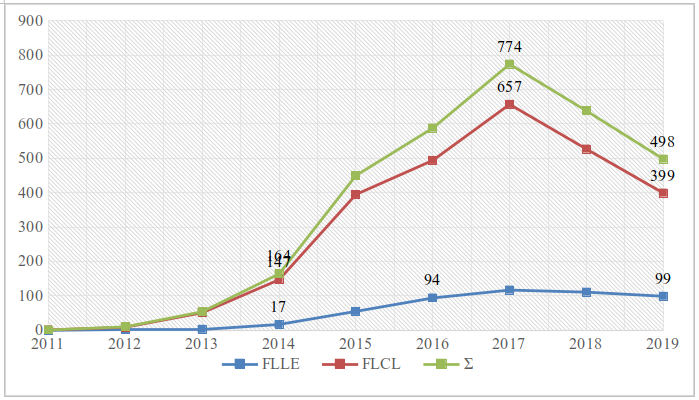
\includegraphics[width=0.85\textwidth]{Fig01.png}
 \caption{Evolution of scientific production.}
 \label{Fig01}
 \source{own elaboration.}
\end{figure}

The predominant language used by researchers in this branch of knowledge is English, both in FLLE and FLCL studies, considerably distanced from the next most widely used language, Spanish (\cref{tbl-tabela-04}).


\begin{table}[htpb]
\caption{Scientific language used.}
\label{tbl-tabela-04}
\centering
\begin{tabular}{lccc}
\toprule
\textbf{Language} & \textbf{FLLE} & \textbf{FLCL} & \textbf{Σ} \\ 
\midrule
English    & 467 & 2525 & 2992 \\ 
Spanish    & 20  & 84   & 104  \\ 
Chinese    & 1   & 41   & 42   \\ 
Portuguese & 4   & 11   & 15   \\ 
Russian    & 1   & 6    & 7    \\ 
German     & -   & 4    & 4    \\ 
Korean     & 2   & 1    & 3    \\ 
Italian    & 1   & 1    & 2    \\ 
French     & -   & 2    & 2    \\ 
Turkish    & -   & 2    & 2    \\ 
Bulgarian  & 1   & 1    & 2    \\ 
Catalan    & -   & 1    & 1    \\ 
Hungarian  & -   & 1    & 1    \\ 
\bottomrule
\end{tabular}
\source{own elaboration.}
\end{table}

The area of knowledge of reference in the studies developed in both terms is that alluding to "Education Educational Research", concentrating there the greatest amount of production. In spite of this, there is a considerable variety of areas that deal with the subject to a lesser extent (\cref{tbl-tabela-05}).

\begin{table}[htpb]
\caption{Areas of knowledge.}
\label{tbl-tabela-05}
\centering
\begin{tabular}{lccc}
\toprule
\textbf{Publication area} & \textbf{FLLE} & \textbf{FLCL} & \textbf{Σ} \\ 
\midrule
Education Educational Research      & 402 & 1859 & 2261 \\ 
Computer Science                    & 59  & 404  & 463  \\ 
Engineering                         & 51  & 293  & 344  \\ 
Social Science other topics         & 11  & 285  & 296  \\ 
Business Economics                  & 9   & 188  & 197  \\ 
Linguistics                         & 22  & 71   & 93   \\ 
Chemistry                           & 11  & 72   & 83   \\ 
Arts Humanites other topics         & 2   & 66   & 68   \\ 
Nursing                             & 12  & 51   & 63   \\ 
Health Care Science Services        & 2   & 48   & 50   \\ 
General Internal Medicine           & 3   & 42   & 45   \\ 
Psychology                          & 5   & 37   & 42   \\ 
Pharmacology Pharmacy               & -   & 39   & 39   \\ 
Science Technology Other Topics     & 9   & 25   & 34   \\ 
Communication                       & 5   & 23   & 28   \\ 
Information Science Library Science & 2   & 25   & 27   \\ 
Biochemistry Molecular Biology      & -   & 26   & 26   \\ 
Literature                          & -   & 24   & 24   \\ 
Cell biology                        & -   & 24   & 24   \\ 
Telecommunications                  & 2   & 22   & 24   \\ 
Dentristry Oral Surgery Medicine    & -   & 21   & 21   \\ 
Art                                 & -   & 15   & 15   \\ 
\bottomrule
\end{tabular}
\source{own elaboration.}
\end{table}

The type of publication used primarily to reveal research findings is congress communications, closely followed by articles. The other publications are poorly represented (\cref{tbl-tabela-06}).

\begin{table}[htpb]
\caption{Type of document.}
\label{tbl-tabela-06}
\centering
\begin{tabular}{lccc}
\toprule
\textbf{Type} & \textbf{FLLE} & \textbf{FLCL} & \textbf{Σ} \\ 
\midrule
Communications     & 210 & 1339 & 1549 \\ 
Papers             & 235 & 1051 & 1286 \\ 
Abstracts          & 6   & 105  & 111  \\ 
Book Chapters      & 23  & 63   & 86   \\ 
Editorial material & 4   & 45   & 49   \\ 
Revisions          & 8   & 44   & 52   \\ 
Letters            & 2   & 15   & 17   \\ 
Early access       & 5   & 4    & 9    \\ 
Newsitem           & -   & 6    & 6    \\ 
Book reviews       & 3   & 3    & 6    \\ 
Corrections        & 1   & 2    & 3    \\ 
Books              & -   & 2    & 2    \\ 
Reissues           & -   & 1    & 1    \\ 
\bottomrule
\end{tabular}
\source{own elaboration.}
\end{table}

The reference institution for the FLCL is the University of North Carolina, while for FLLE it is the National Taiwan University of Science Technology. The rest of the institutions have a medium or low incidence in scientific production (\cref{tbl-tabela-07}).

\begin{table}[htpb]
\caption{Institutions.}
\label{tbl-tabela-07}
\centering
\begin{tabular}{lccc}
\toprule
\textbf{Denomination} & \textbf{FLLE} & \textbf{FLCL} & \textbf{Σ} \\ 
\midrule
University of North Carolina                          & 4  & 48 & 52 \\ 
University of Carolina Systems                        & -  & 31 & 31 \\ 
University of Hong Kong                               & 11 & 20 & 30 \\ 
Harvard University                                    & 1  & 29 & 30 \\ 
State University System of Florida                    & 1  & 28 & 29 \\ 
National Taiwan University of Science Technology      & 14 & 13 & 27 \\ 
University of North Carolina Chapel Hill              & 1  & 25 & 26 \\ 
Pennsylvania Common Wealth System of Higher Education & 1  & 25 & 26 \\ 
University System of Georgia                          & -  & 22 & 22 \\ 
Universidad Politécnica de Madrid                     & 2  & 20 & 22 \\ 
Universitat Politécnica de Valencia                   & 5  & 17 & 22 \\ 
National Taiwan Normal University                     & 5  & 15 & 20 \\ 
University of Sydney                                  & 6  & 14 & 20 \\ 
Universidad de Zaragoza                               & 6  & 15 & 21 \\ 
California State University System                    & 2  & 16 & 18 \\ 
Bohai University                                      & -  & 17 & 17 \\ 
University of Michigan System                         & -  & 17 & 17 \\ 
Monash University                                     & 1  & 16 & 17 \\ 
Universidad de Extremadura                            & 2  & 15 & 17 \\ 
Polytechnic Institute of Porto                        & 3  & 14 & 17 \\ 
State University of New York Suny System              & -  & 16 & 16 \\ 
University of Michigan                                & -  & 16 & 16 \\ 
Ohio State University                                 & -  & 15 & 15 \\ 
Va Boston Healthcare System                           & 1  & 13 & 14 \\ 
Northeast Normal University China                     & -  & 13 & 13 \\ 
MEF Universitesi                                      & 8  & 1  & 9  \\ 
\bottomrule
\end{tabular}
\source{own elaboration.}
\end{table}

The main author in FLLE is Hwang, G.J., while in FLCL there are several authors with a high output, such as Keengwe, J., Oigara, J.N. and Onchwari, G (\cref{tbl-tabela-08}). It also reflects the presence of authors who develop works using both terms.

\begin{table}[htpb]
\caption{Most prolific authors.}
\label{tbl-tabela-08}
\centering
\begin{tabular}{lccc}
\toprule
\textbf{Authors}   & \textbf{FLLE} & \textbf{FLCL} & \textbf{Σ} \\ 
\midrule
Hwang, G.J.        & 19            & 10            & 29         \\ 
Keengwe, J.        & -             & 18            & 18         \\ 
Oigara, J.N.       & -             & 17            & 17         \\ 
Onchwari, G.       & -             & 17            & 17         \\ 
Zainuddin, Z.      & 4             & 9             & 13         \\ 
Jeong, J.S.        & 1             & 11            & 12         \\ 
McLaughlin, J.E.   & 1             & 11            & 12         \\ 
Scheg, A.G.        & 3             & 9             & 12         \\ 
Liu, Y.            & -             & 11            & 11         \\ 
Canada-Canada, F.  & 1             & 9             & 10         \\ 
González-Gómez, D. & 1             & 9             & 10         \\ 
Wang, L.           & 1             & 9             & 10         \\ 
Hew, K.F.          & 4             & 6             & 10         \\ 
Lo, C.K.           & 4             & 6             & 10         \\ 
Chen, N.S.         & 2             & 7             & 9          \\ 
Artal-Sevil, J.S.  & 3             & 6             & 9          \\ 
Hung, H.T.         & 3             & 6             & 9          \\ 
Li, Y.             & -             & 8             & 8          \\ 
\bottomrule
\end{tabular}
\source{own elaboration.}
\end{table}

Regarding the source of publication (\cref{tbl-tabela-09}), the collection "Advances in Social Science Education and Humanities Research", is the one that most publishes on FLCL, while on the FLLE concept is the collection "INTED Proceedings".

\begin{table}[htpb]
\caption{Most prolific authors.}
\label{tbl-tabela-09}
\centering
\begin{tabular}{lccc}
\toprule
\textbf{Denomination} & \textbf{FLLE} & \textbf{FLCL} & \textbf{Σ} \\ 
\midrule
Advances in Social Science Education and Humanities Research       & 5  & 174 & 179 \\ 
INTED Proceedings                                                  & 47 & 101 & 148 \\ 
EDULEARN Proceedings                                               & 40 & 104 & 144 \\ 
ICERI Proceedings                                                  & 23 & 72  & 95  \\ 
\begin{tabular}[c]{@{}l@{}}12TH International Technology Education and \\ Development Conference INTED\end{tabular} &
  17 &
  32 &
  49 \\ 
ACSR Advances in computer Science Research                         & -  & 46  & 46  \\ 
Destech Transactions on Social Science Education and Human Science & 2  & 41  & 43  \\ 
Frontiers in Education Conference                                  & 3  & 40  & 43  \\ 
\begin{tabular}[c]{@{}l@{}}EDULEARN 8TH International Conference on Education \\ and New Learning Technology\end{tabular} &
  13 &
  29 &
  42 \\ 
\begin{tabular}[c]{@{}l@{}}INTED 2017 11TH International technology education and \\ Development Conference\end{tabular} &
  14 &
  27 &
  41 \\ 
Lecture Notes in Managements Science                               & 3  & 36  & 39  \\ 
\begin{tabular}[c]{@{}l@{}}10TH International Conference of Education Research and \\ Innovation\end{tabular} &
  10 &
  23 &
  33 \\ 
Educational Technology Society                                     & 7  & 23  & 30  \\ 
Computers Education                                                & 7  & 22  & 29  \\ 
\begin{tabular}[c]{@{}l@{}}INTED 2016 10th International Technology Education and \\ Development Conference\end{tabular} &
  9 &
  20 &
  29 \\ 
Abstracts of Papers of the American Chemical Society               & 2  & 26  & 28  \\ 
Journal Of Chemical Education                                      & 2  & 26  & 28  \\ 
\begin{tabular}[c]{@{}l@{}}EDULEARN 15 7TH International Conference on Education and \\ New Learning Technologies\end{tabular} &
  4 &
  22 &
  26 \\ 
American Journal of Pharmaceutical Education                       & -  & 25  & 25  \\ 
Lecture Notes in Computer Science                                  & 3  & 20  & 23  \\ 
Advances in intelligent systems research                           & 1  & 21  & 22  \\ 
Faseb journal                                                      & -  & 21  & 21  \\ 
International Journal of Emerging Technologies in Learning         & 1  & 20  & 21  \\ 
Advancesin Education Research                                      & -  & 19  & 19  \\ 
\bottomrule
\end{tabular}
\source{own elaboration.}
\end{table}

The country of reference in the scientific production on both concepts is the United States, although China follows closely, especially in the production concerning FLCL (\cref{tbl-tabela-10}).

\begin{table}[htpb]
\caption{Relationship of countries with production on the theme.}
\label{tbl-tabela-10}
\centering
\begin{tabular}{lccc}
\toprule
\textbf{Country} & \textbf{FLLE} & \textbf{FLCL} & \textbf{Σ} \\
\midrule
United States & 89 & 741 & 830 \\ 
China         & 32 & 682 & 714 \\ 
Spain         & 48 & 196 & 244 \\ 
Taiwan        & 51 & 115 & 166 \\ 
Australia     & 25 & 98  & 123 \\ 
England       & 23 & 72  & 95  \\ 
Turkey        & 27 & 42  & 69  \\ 
Canada        & 8  & 56  & 64  \\ 
Malaysia      & 14 & 42  & 56  \\ 
South Korea   & 33 & 22  & 55  \\ 
Germany       & 4  & 50  & 54  \\ 
Japan         & 17 & 27  & 44  \\ 
Italy         & 13 & 28  & 41  \\ 
Indonesia     & 8  & 27  & 35  \\ 
Norway        & 5  & 29  & 34  \\ 
Russia        & 6  & 28  & 34  \\ 
Brazil        & 2  & 29  & 31  \\ 
Portugal      & 7  & 25  & 32  \\ 
South Africa  & 2  & 22  & 24  \\ 
India         & 3  & 20  & 23  \\ 
Singapore     & 4  & 19  & 23  \\ 
Thailand      & 5  & 17  & 22  \\ 
Netherlands   & 3  & 17  & 20  \\ 
Sweden        & -  & 18  & 18  \\ 
\bottomrule
\end{tabular}
\source{own elaboration.}
\end{table}

The most outstanding references, both in FLLE (\cref{tbl-tabela-11}) and in FLCL (\cref{tbl-tabela-12}), show significant differences in relation to the importance and incidence in the scientific community itself, resulting in a higher citation index in the studies covered by the term FLCL.

\begin{table}[htpb]
\caption{FLLE: most-cited articles.}
\label{tbl-tabela-11}
\centering
\begin{tabular}{p{0.7\textwidth}c}
\toprule
\textbf{References} & \textbf{Citations} \\ 
\midrule
CHEN, Y.L., WANG, Y.P., KINSHUK, \& CHEN, N.S. (2014). Is FLIP enough? Or should we use the FLIPPED model instead?. \textit{Computers \& Education}, 79, 16--27. & 165 \\ 
\noalign{\vskip 1ex}
TRAVIS, R. (2014). Student perceptions toward flipped learning: New methods to increase interaction and active learning in economics. \textit{International review of Economics Education}, 17, 74--84. & 119 \\ 
\noalign{\vskip 1ex}
LAI, C.L., \& HWANG, G.J. (2016). A self-regulated flipped classroom approach to improving students' learning performance in a mathematics course. \textit{Computers \& Education}, 100, 126--140. & 104 \\ 
\noalign{\vskip 1ex}
HWANG, G.J., LAI, C.L., \& WANG, S.Y. (2015). Seamless flipped learning: a mobile technology-enhanced flipped classroom with effective learning strategies. \textit{Journal of computers in education}, 2(4), 449--473. &  96 \\
\noalign{\vskip 1ex}
SEERY, M.K. (2015). Flipped learning in higher education chemistry: emerging trends and potential directions. \textit{Chemistry education research and practice}, 16(4), 758--768. & 72 \\ 
\bottomrule
\end{tabular}
\source{own elaboration.}
\end{table}

\begin{table}[htpb]
\caption{FLCL: most-cited articles.}
\label{tbl-tabela-12}
\centering
\begin{tabular}{p{0.7\textwidth}c}
\toprule
\textbf{References} & \textbf{Citations} \\ 
\midrule
O´FLAHERTY, J., \& PHILLIPS, C. (2015). The use of flipped classrooms in higher education: A scoping review. \textit{Internet and Higher education}, 25, 85--95. doi: 10.1016/j.iheduc.2015.02.002 & 413 \\ 
\noalign{\vskip 1ex}
MCLAUGHLIN, JE, ROTH, MT, GLATT, DM, GHARKHOLONARECHE, N., DAVIDSON, C.A., GRIFFIN, L.M., ESSERMAN, D.A., \& MUMPER, R.J. (2014). The flipped classroom: a course redesign to Foster learning and engagement in a health professions school. \textit{Academic Medicine}, 89(2), 236--243. & 375 \\ 
\noalign{\vskip 1ex}
ABEYSEKERA, L., \& DAWSON, P. (2015). Motivation and cognitive load in the flipped classroom: definition, rationale and a call for research. \textit{Higher Education Research \& Development}, 34(1), 1--14. & 310 \\
\noalign{\vskip 1ex}
MASON, G.S., SHUMAN, T.R., \& KATHLEEN, E. (2013). Comparing the effectiveness of an inverted classroom to a traditional classroom in an upper-division engineering course. \textit{IEEE Transactions on Education}, 56(4), 430--435. &  293 \\ 
\noalign{\vskip 1ex}
DAVIES, R.S., DEAN, D.L., \& BALL, N. (2013). Flipping the classroom and instructional technology integration in a college-level information systems spreadsheet course. \textit{Etr\&D-Educational Technology research} development, 61(4), 563--580 & 258 \\ 
\bottomrule
\end{tabular}
\source{own elaboration.}
\end{table}

%italico e maiúsculas

\subsection{Structural and thematic development}\label{sec-structural}
With respect to the continuity produced in the keywords in the delimited periods, it shows a more established thematic predominance in FLCL than in FLLE, given that the percentage of similarity between dates is higher in the former than in the latter, there being similarities between the years 2017-2018 and 2018-2019. Likewise, an evolution of key words is observed from the beginning established until the year 2018, in which there is a slight decrease in FLCL and --very similar-- in FLLE (\cref{Fig02}).

\begin{figure}[htbp]
 \centering
 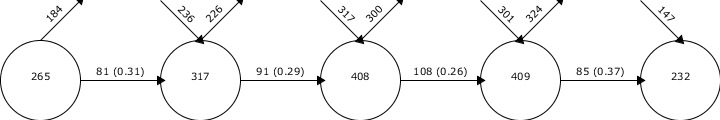
\includegraphics[width=0.8\textwidth]{Fig02.png}
 \caption{Continuity of keywords between contiguous periods. Note: (a) FLCL; (b) FLLE.}
 \label{Fig02}
 \source{own elaboration. }
\end{figure}

As shown in \Cref{tbl-tabela-13}, in relation to FLCL, there is a thematic plurality in the different established periods, given the variety in the research reported in this field of knowledge, but with a continuous line between periods, if we bear in mind the different bibliometric indicators. Specifically, in 2014 and 2015 the concept with the most indices was "blended learning", while from 2016 to 2018 the "flipped classroom" theme is included in the witness. It is in 2019 that a radical change in research perspectives is shown, with new topics and new lines of study being offered.

\begin{longtable}{lllllll}
\caption{Thematic performance in FLCL.}
\label{tbl-tabela-13}
\\
\multicolumn{7}{c}{\textbf{Period 2011-2013}} \\ 
\toprule
\textbf{Denomination}       & \textbf{Works} & \textbf{h-index} & \textbf{g-index} & \textbf{hg-index} & \textbf{q2-index} & \textbf{Citations} \\ 
\toprule
Education                   & 10             & 5                & 7                & 5.92              & 17.75             & 481                \\ 
Classroom                   & 2              & 1                & 1                & 1                 & 2.65              & 7                  \\ 
Problem based learning      & 2              & 2                & 2                & 2                 & 11.22             & 101                \\ 
\bottomrule 
\noalign{\vskip 3ex} 
\multicolumn{7}{c}{\textbf{Period 2014}} \\ 
\toprule
\textbf{Denomination}       & \textbf{Works} & \textbf{h-index} & \textbf{g-index} & \textbf{hg-index} & \textbf{q2-index} & \textbf{Citations} \\ 
\midrule
Model                       & 4              & 4                & 4                & 4                 & 18.97             & 242                \\ 
On-line                     & 7              & 5                & 6                & 5.48              & 9.22              & 263                \\ 
Inverted classroom          & 16             & 5                & 8                & 6.32              & 12.25             & 406                \\ 
Blended learning            & 12             & 5                & 8                & 6.32              & 20.12             & 472                \\ 
MOOC                        & 2              & 0                & 0                & 0                 & 0                 & 0                  \\ 
School                      & 2              & 1                & 1                & 1                 & 1.41              & 2                  \\ 
\bottomrule

\noalign{\vskip 3ex}
\multicolumn{7}{c}{\textbf{Period 2015}} \\ 
\toprule
\textbf{Denomination}       & \textbf{Works} & \textbf{h-index} & \textbf{g-index} & \textbf{hg-index} & \textbf{q2-index} & \textbf{Citations} \\ 
\midrule
Quality                     & 3              & 1                & 1                & 1                 & 4.69              & 22                 \\ 
First Year Undergraduate    & 10             & 8                & 10               & 8.94              & 11.31             & 166                \\ 
Blended learning            & 42             & 12               & 20               & 15.49             & 18                & 433                \\ 
Students                    & 16             & 9                & 14               & 11.22             & 19.21             & 855                \\ 
Active learning             & 13             & 7                & 13               & 9.54              & 10.91             & 264                \\ 
Technology                  & 11             & 2                & 3                & 2.45              & 3.74              & 10                 \\ 
Physiology                  & 3              & 2                & 2                & 2                 & 7.48              & 30                 \\ 
Collaboration               & 3              & 0                & 0                & 0                 & 0                 & 0                  \\ 
MOOC                        & 4              & 2                & 3                & 2.45              & 4.47              & 13                 \\ 
\bottomrule

\noalign{\vskip 3ex}
\multicolumn{7}{c}{\textbf{Period 2016}} \\ 
\toprule
\textbf{Denominación}       & \textbf{Works} & \textbf{h-index} & \textbf{g-index} & \textbf{hg-index} & \textbf{q2-index} & \textbf{Citations} \\ 
\midrule
Flipped classroom           & 126            & 16               & 25               & 20                & 22.27             & 799                \\ 
Performance                 & 21             & 11               & 17               & 13.67             & 14.46             & 319                \\ 
Student performance         & 15             & 8                & 15               & 10.95             & 18.55             & 364                \\ 
Classroom                   & 10             & 3                & 10               & 5.48              & 9.49              & 229                \\ 
Design                      & 4              & 4                & 4                & 4                 & 5.66              & 40                 \\ 
Learning                    & 5              & 2                & 3                & 2.45              & 4.9               & 25                 \\ 
College English             & 5              & 0                & 0                & 0                 & 0                 & 0                  \\ 
\bottomrule

\noalign{\vskip 3ex}
\multicolumn{7}{c}{\textbf{Period 2017}} \\ 
\toprule
\textbf{Denomination}       & \textbf{Works} & \textbf{h-index} & \textbf{g-index} & \textbf{hg-index} & \textbf{q2-index} & \textbf{Citations} \\ 
\midrule
Medical education           & 28             & 11               & 17               & 13.67             & 12.85             & 328                \\ 
Flipped classroom           & 201            & 12               & 19               & 15.1              & 17.32             & 600                \\ 
Experience                  & 25             & 8                & 13               & 10.2              & 11.31             & 193                \\ 
Classroom                   & 21             & 4                & 6                & 4.9               & 6.63              & 52                 \\ 
Flipped learning            & 17             & 5                & 9                & 6.71              & 6.71              & 83                 \\ 
Learning                    & 5              & 2                & 2                & 2                 & 2.45              & 6                  \\ 
Design                      & 7              & 2                & 4                & 2.83              & 3.74              & 17                 \\ 
Student centered learning   & 3              & 0                & 0                & 0                 & 0                 & 0                  \\ 
MOOC                        & 11             & 3                & 4                & 3.46              & 3.87              & 20                 \\ 
\bottomrule

\noalign{\vskip 3ex}
\multicolumn{7}{c}{\textbf{Period 2018}} \\
\toprule
\textbf{Denomination}       & \textbf{Works} & \textbf{h-index} & \textbf{g-index} & \textbf{hg-index} & \textbf{q2-index} & \textbf{Citations} \\ 
\midrule
Flipped classroom           & 163            & 7                & 9                & 7.94              & 7.48              & 246                \\ 
Impact                      & 13             & 4                & 5                & 4.47              & 4.9               & 36                 \\ 
Motivation                  & 31             & 3                & 6                & 4.24              & 5.2               & 59                 \\ 
Skills                      & 22             & 3                & 4                & 3.46              & 3.87              & 36                 \\ 
Perceptions                 & 16             & 4                & 4                & 4                 & 4.9               & 34                 \\ 
Outcomes                    & 8              & 3                & 5                & 4.24              & 6.48              & 47                 \\ 
Flipped learning            & 6              & 1                & 1                & 1                 & 1                 & 3                  \\ 
Learning management systems & 4              & 1                & 1                & 1                 & 1                 & 1                  \\ 
Learners                    & 4              & 1                & 2                & 1.41              & 3                 & 10                 \\ 
College English             & 4              & 1                & 1                & 1                 & 2                 & 4                  \\ 
\bottomrule

\noalign{\vskip 3ex}
\multicolumn{7}{c}{\textbf{Period 2019}} \\
\toprule
\textbf{Denomination}       & \textbf{Works} & \textbf{h-index} & \textbf{g-index} & \textbf{hg-index} & \textbf{q2-index} & \textbf{Citations} \\ 
\midrule
Motivation                  & 41             & 4                & 6                & 4.9               & 6.32              & 50                 \\ 
Design                      & 58             & 4                & 6                & 4.9               & 6.63              & 63                 \\ 
Curriculum                  & 21             & 2                & 5                & 3.16              & 6.48              & 31                 \\ 
Technology                  & 23             & 2                & 3                & 2.45              & 3.16              & 12                 \\ 
Model                       & 16             & 2                & 3                & 2.45              & 3.16              & 11                 \\ 
Active-learning             & 14             & 2                & 2                & 2                 & 2                 & 6                  \\ 
Perceptions                 & 14             & 2                & 2                & 2                 & 2.83              & 7                  \\ 
Principles                  & 5              & 1                & 1                & 1                 & 1.41              & 2                  \\ 
Medical education           & 6              & 0                & 0                & 0                 & 0                 & 0                  \\ 
Student performance         & 6              & 1                & 1                & 1                 & 1.41              & 2                  \\ 
Learning strategies         & 2              & 1                & 1                & 1                 & 2                 & 4                  \\ 
ICT                         & 3              & 1                & 1                & 1                 & 1.41              & 2                  \\ 
Strategies                  & 3              & 1                & 1                & 1                 & 1                 & 2                  \\ 
Courses                     & 2              & 0                & 0                & 0                 & 0                 & 0                  \\ 
\bottomrule
\source{own elaboration.}
\end{longtable}

With respect to FLLE, like its homonym, it also offers thematic varieties in the various defined periods (\cref{tbl-tabela-14}), but with a line established if bibliometric indicators are taken into account. From 2012 to 2016, the main concept is "flipped classroom", becoming in 2017 "university" and in 2018 "flipped learning". In the data recorded to date, the year 2019 offers new perspectives and trends in research, focusing on "performance", “classroom model” and "motivation".

\begin{longtable}{lllllll}
\caption{Thematic performance in FLLE.}
\label{tbl-tabela-14}
\\
\multicolumn{7}{c}{\textbf{Period 2012-2015}} \\ 
\toprule
\textbf{Denomination} & \textbf{Works} & \textbf{h-index} & \textbf{g-index} & \textbf{hg-index} & \textbf{q2-index} & \textbf{Citations} \\
\midrule
Classroom &  6 &  3 & 4 & 3.46 & 11.09 & 118 \\ 
Flipped classroom &  20 & 3 & 9 &  5.2 & 5.2 & 96 \\ 
Environment & 3 & 3 & 3 & 3 & 14.9 & 220 \\
Pedagogy & 2 & 1 & 1 & 1 & 1.41 & 2 \\
Organic-Chemistry &  3 & 3 & 3 & 3 & 6.71 & 90 \\
\bottomrule
\noalign{\vskip 3ex}
\multicolumn{7}{c}{\textbf{Period 2016}} \\ 
\toprule
\textbf{Denomination} & \textbf{Works} & \textbf{h-index} & \textbf{g-index} & \textbf{hg-index} & \textbf{q2-index} & \textbf{Citations} \\ 
\midrule
Achievement & 3 & 3 & 3 & 3 & 11.87 & 113 \\ 
Environment & 3 & 3 & 3 & 3 & 8.66 & 112 \\ 
Engineering education & 2 & 1 & 1 & 1 & 1 & 1 \\
Flipped classroom & 11 & 5 & 10 & 7.07 & 8.06 & 108 \\
Experience &  2 & 2 & 2 & 2 & 9.7 & 53 \\
\bottomrule
\noalign{\vskip 3ex}
\multicolumn{7}{c}{\textbf{Period 2017}} \\ 
\toprule
\textbf{Denomination} & \textbf{Works} & \textbf{h-index} & \textbf{g-index} & \textbf{hg-index} & \textbf{q2-index} & \textbf{Citations} \\
\midrule
On line academic help seeking &  2 &  2 &  2 &  2 &  3.16 &  8 \\ 
Student Centered learning &  6 & 4 & 6 &  4.9 &  5.66 &  36 \\ 
Motivation &   6 &  5 &  5 &  5 &  6.32 &  63 \\ 
University &  7 &  6 &  7 &  6.48 &  7.75 &  73 \\ 
Students &  15 &  5 &  8 &  6.32 &  7.42 &  66 \\ 
Student performance &  8 &  4 &  6 &  4.9 &  6.32 &  45 \\ 
Flipped learning &  21 &  5 &  7 &  5.92 &  6.32 &  65 \\ 
Education &  3 &  1 &  1 &  1 &  1 &  1 \\ 
Mobile technology &  2 &  1 &  1 &  1 &  2.65 &  7 \\ 
Collaborative learning &  2 &  1 &  1 &  1 &  1.41 & 2 \\ 
\bottomrule
\noalign{\vskip 3ex}
\multicolumn{7}{c}{\textbf{Period 2018}} \\
\toprule
\textbf{Denomination} & \textbf{Works} & \textbf{h-index} & \textbf{g-index} & \textbf{hg-index} & \textbf{q2-index} & \textbf{Citations} \\
\midrule
Middle school &  5 & 2 & 2 & 2 & 4.47 & 14 \\ 
Percepctions &  6 & 1 & 1 & 1 & 2 & 4 \\ 
Design & 9 & 3 & 4 & 3.46 & 3.87 & 22 \\ 
Learning analytics &  7 & 1 & 2 & 1.41 & 2 & 7 \\
Educational technology &  4 & 1 & 2 & 1.41 & 2 & 5 \\
Flipped learning & 30 & 3 &  5 & 3.87 & 3.87 & 31 \\ 
Flipped classroom & 11 & 2 & 3 & 2.45 & 3.16 & 12 \\
Video &  2 & 0 & 0 & 0 & 0 & 0 \\
Learners & 2 &  1 & 1 & 1 & 1.73 & 3 \\
Innovation & 2 & 0 & 0 & 0 & 0 & 0 \\
\bottomrule
\noalign{\vskip 3ex}
\multicolumn{7}{c}{\textbf{Period 2019}} \\ 
\toprule
\textbf{Denomination} & \textbf{Works} & \textbf{h-index} & \textbf{g-index} & \textbf{hg-index} & \textbf{q2-index} & \textbf{Citations} \\
\midrule
Classroom model & 5 & 2 & 2 & 2 & 5.83 & 19 \\ 
Performance & 15 & 2 & 4 & 2.83 & 5.83 & 22 \\ 
Satisfaction & 7 & 2 & 2 & 2 & 2.45 & 6 \\ 
Flipped learning & 20 & 1 & 1 & 1 & 1.73 & 3 \\ 
Motivation & 6 & 2 & 2 & 2 & 5.83 & 19 \\ 
Medical Education & 2 & 0 & 0 & 0 & 0 & 0 \\
Learners & 3 & 1 & 1 & 1 & 1 & 1 \\ 
\bottomrule
\source{own elaboration.}
\end{longtable}

Analyzing the different diagrams of the periods established in the FLCL, it can be observed that "flipped classroom" is the theme that has been the most established in time, given that it has been a relevant theme from 2016 to 2018, continuing -in the same way- in the studies that are developed, focused mainly on "Blended learning", "Higher education", "students" and "active learning". In recent years (2018-2019), there has been a growing trend in aspects related to motivation, impact on students and performance. As shown in both periods, attention should be paid to the topics "ICT", "strategies", "student performance" and "medical education", as they are concepts whose durability implies a mystery, and may disappear in the future or emerge as driving themes (\cref{fig03a,fig03b,fig03c,fig03d,fig03e,fig03f,fig03g}).

\begin{figure}[htbp]
 \begin{minipage}{.45\textwidth}
 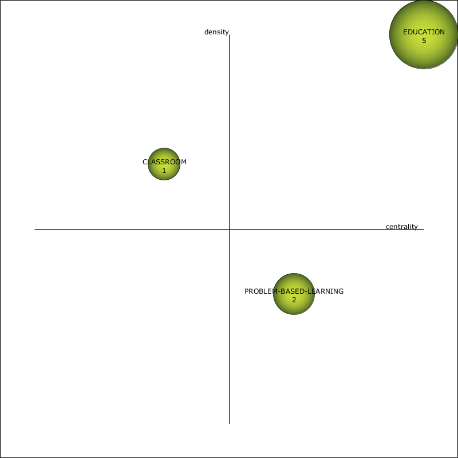
\includegraphics[width=\textwidth]{Fig03a.png}
 \subcaption{Period 2011--2013.}\label{fig03a}
 \end{minipage}
 \hfill
 \begin{minipage}{.45\textwidth}
 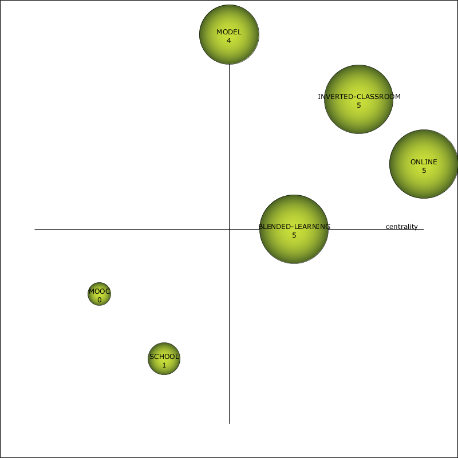
\includegraphics[width=\textwidth]{Fig03b.png}
 \subcaption{Period 2014.}\label{fig03b}
 \end{minipage}
 \par\vspace{2ex}
 \begin{minipage}{.45\textwidth}
 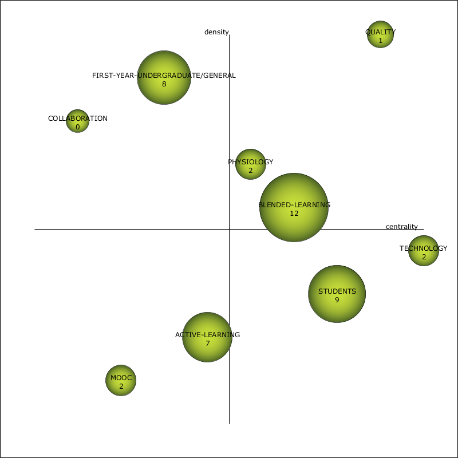
\includegraphics[width=\textwidth]{Fig03c.png}
 \subcaption{Period 2015.}\label{fig03c}
 \end{minipage}
 \hfill
 \begin{minipage}{.45\textwidth}
 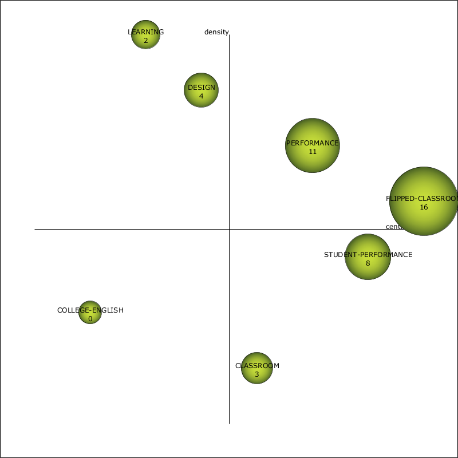
\includegraphics[width=\textwidth]{Fig03d.png}
 \subcaption{Period 2016.}\label{fig03d}
 \end{minipage}
 \par\vspace{2ex}
 \begin{minipage}{.45\textwidth}
 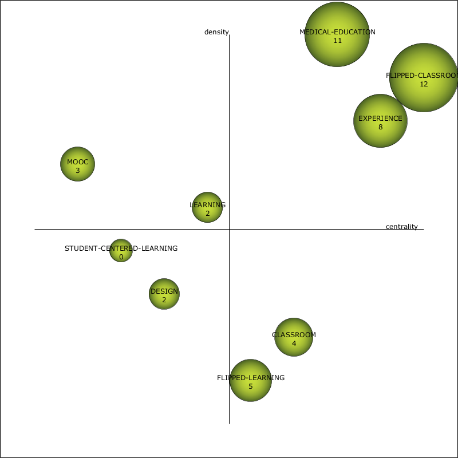
\includegraphics[width=\textwidth]{Fig03e.png}
 \subcaption{Period 2017.}\label{fig03e}
 \end{minipage}
 \hfill
 \begin{minipage}{.45\textwidth}
 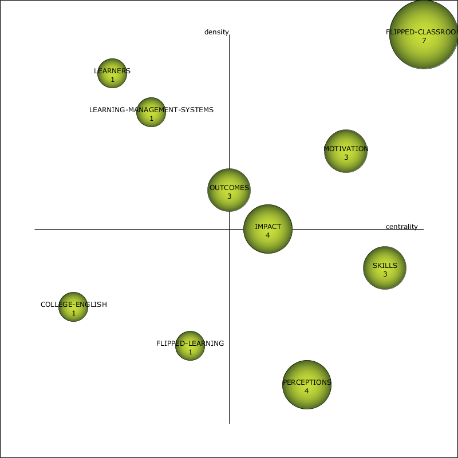
\includegraphics[width=\textwidth]{Fig03f.png}
 \subcaption{Period 2018.}\label{fig03f}
 \end{minipage}
\caption{Strategic diagram by FLCL h-index.}
\label{fig03}
\source{own elaboration.}
\end{figure}
 
\begin{figure}[htbp]\ContinuedFloat
 \begin{minipage}{.45\textwidth}
 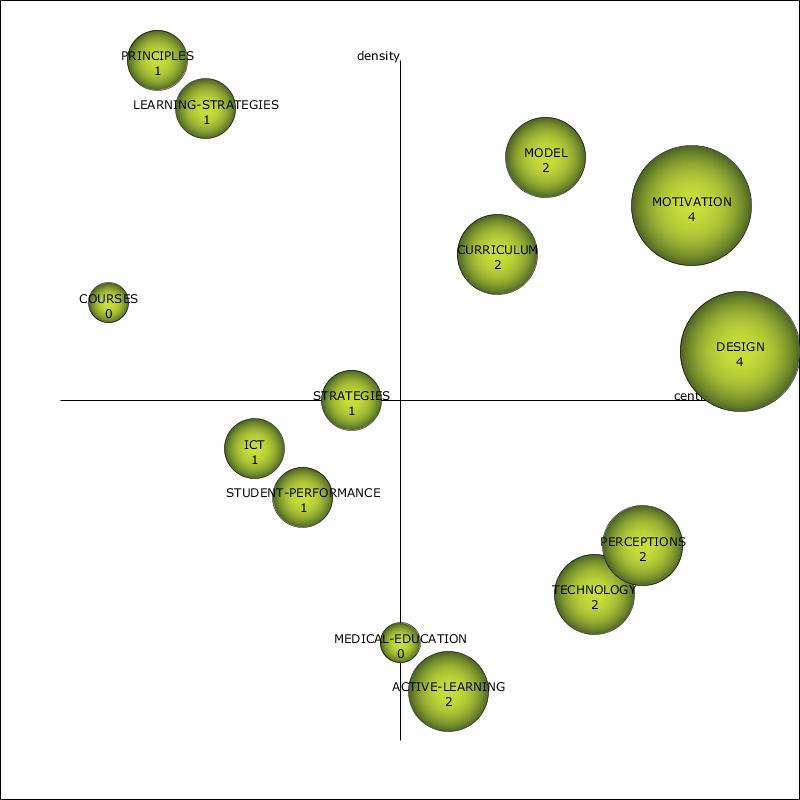
\includegraphics[width=\textwidth]{Fig03g.png}
 \subcaption{Period 2019.}\label{fig03g}
 \end{minipage}
 \hfill
 \begin{minipage}{.45\textwidth}
  \hfill
 \end{minipage}
 \caption{Strategic diagram by FLCL h-index.}
 \label{fig03}
 \source{own elaboration.}
\end{figure}

In the strategic diagrams of the dates configured for FLLE –in contrast to what happened with FLLE– there is no motor theme settled in time, showing changes in each of the periods. The only theme that repeats as the driving theme is "motivation", which appears in 2017 and 2019, although with different research perspectives, given that in 2017, the research focuses on oral training, technology, reading, class models, language students, collaboration and acceptance by users; while in 2019, it is associated with classroom approach, blended learning, self regulated learning perceptions e-learning, skills and achievement. For the coming years, the themes of "motivation" and "learners" should be taken into consideration, given that their location in the diagram places them as emerging or disappearing themes (\cref{fig04a,fig04b,fig04c,fig04d}).



\begin{figure}[htbp]
 \begin{minipage}{.45\textwidth}
 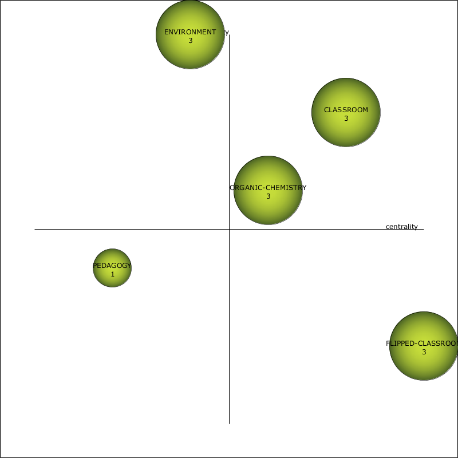
\includegraphics[width=\textwidth]{Fig04a.png}
 \subcaption{Period 2012--2015.}\label{fig04a}
 \end{minipage}
 \hfill
 \begin{minipage}{.45\textwidth}
 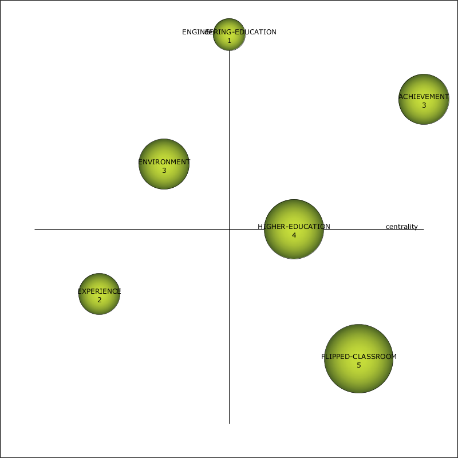
\includegraphics[width=\textwidth]{Fig04b.png}
 \subcaption{Period 2016.}\label{fig04b}
 \end{minipage}
 \par\vspace{2ex}
 \begin{minipage}{.45\textwidth}
 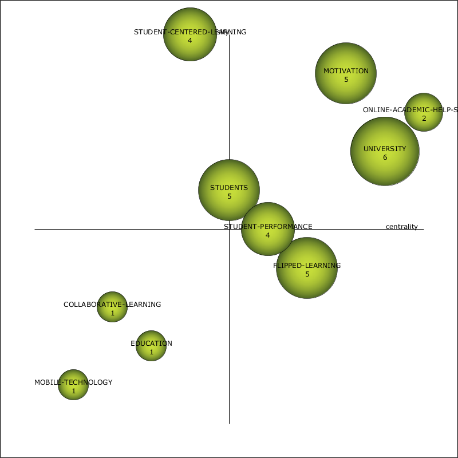
\includegraphics[width=\textwidth]{Fig04c.png}
 \subcaption{Period 2017.}\label{fig04c}
 \end{minipage}
 \hfill
 \begin{minipage}{.45\textwidth}
 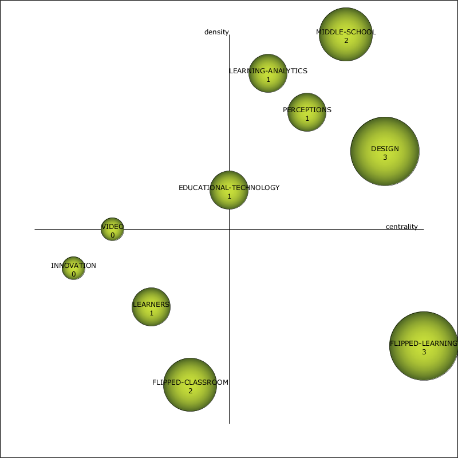
\includegraphics[width=\textwidth]{Fig04d.png}
 \subcaption{Period 2018.}\label{fig04d}
 \end{minipage}
 \par\vspace{2ex}
 \begin{minipage}{.45\textwidth}
 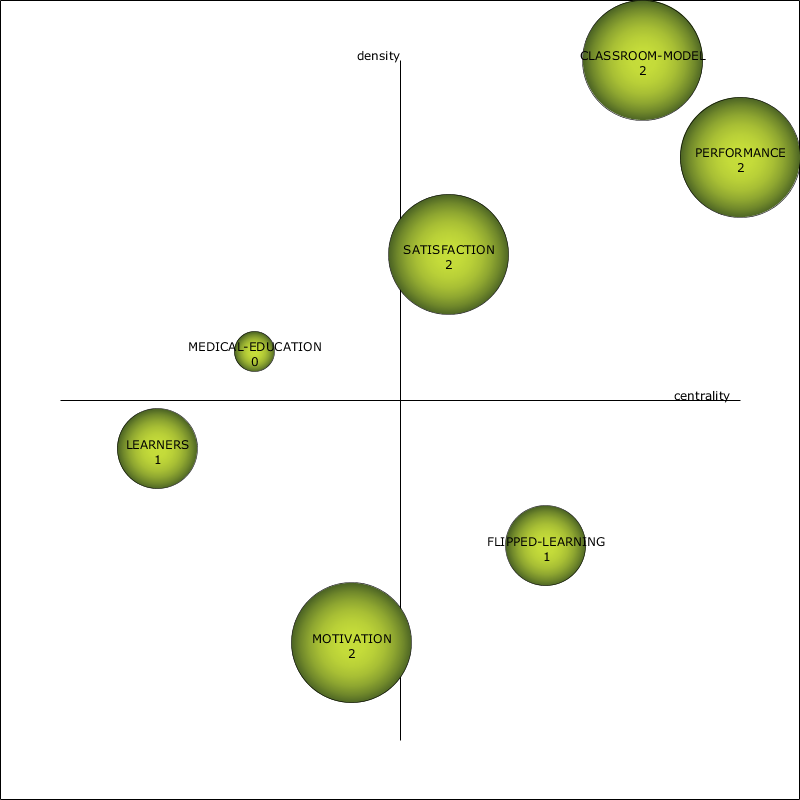
\includegraphics[width=\textwidth]{Fig04e.png}
 \subcaption{Period 2019.}\label{fig04e}
 \end{minipage}
 \hfill
 \begin{minipage}{.45\textwidth}
 \hfill
 \end{minipage}
\caption{Strategic diagram by FLLE h-index.}
\label{fig04}
\source{own elaboration.}
\end{figure}



\subsection{Thematic evolution of terms}\label{sec-thematic}
Considering the thematic evolution shown in \cref{fig05a,fig05b}, attention should be paid to the type of line of connections made. The solid line shows a conceptual relationship and the dashed line reflects a non-conceptual relationship, given that the connection is through key words.


\begin{figure}[htbp]
 \begin{minipage}{\textwidth}
 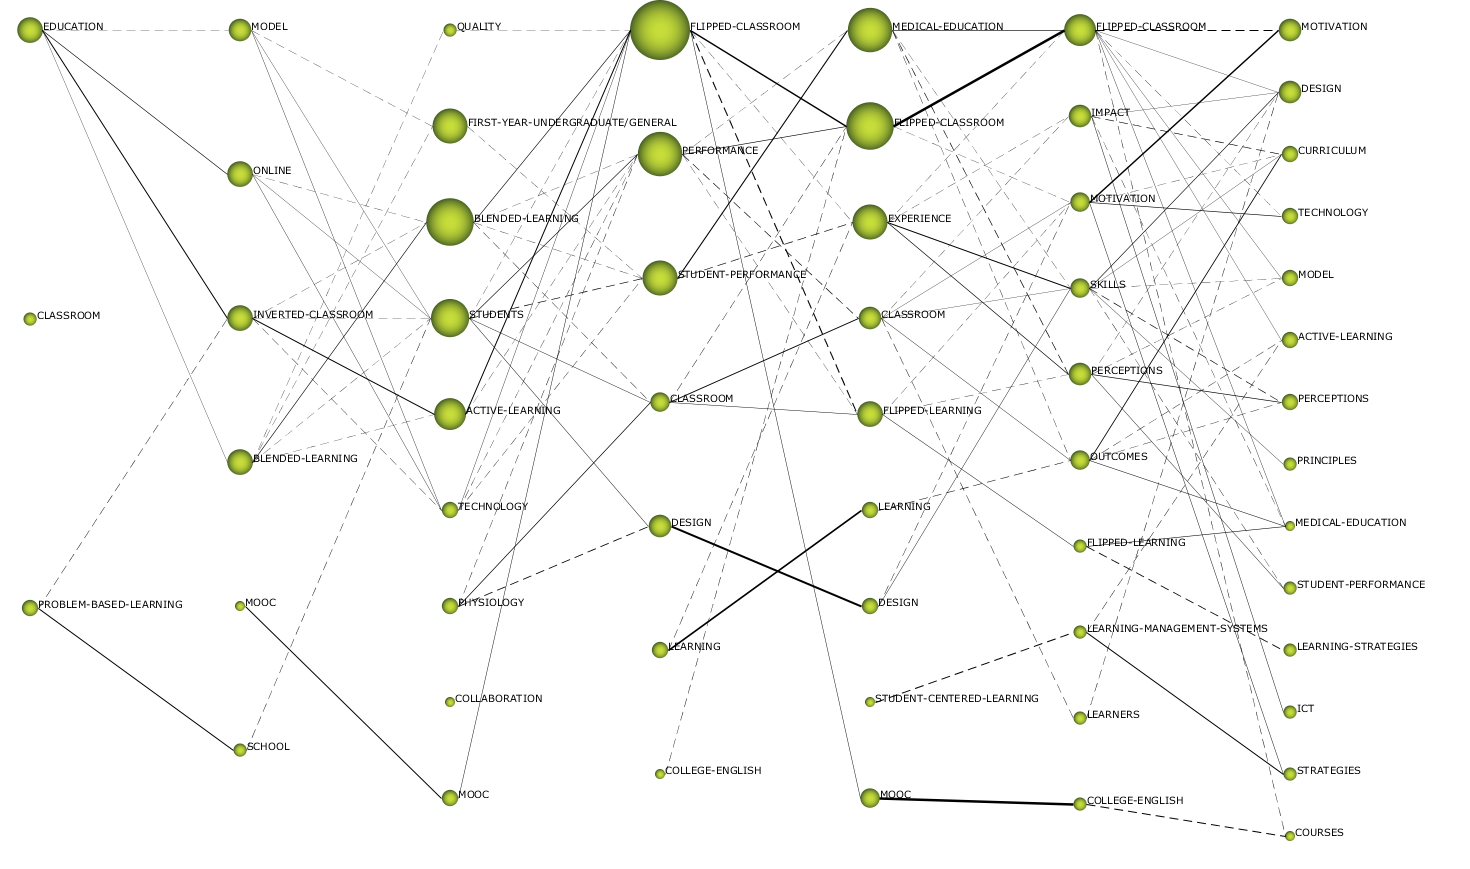
\includegraphics[width=\textwidth]{Fig05a.png}
 \subcaption{FLCL.}\label{fig05a}
 \end{minipage}
 \\
 \begin{minipage}{\textwidth}
 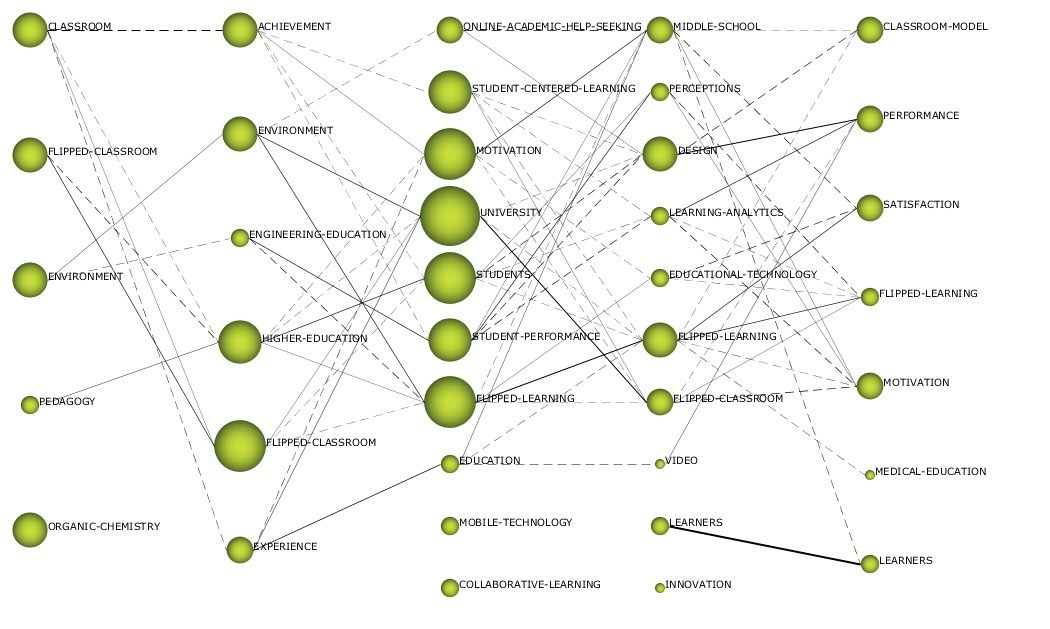
\includegraphics[width=\textwidth]{Fig05b.png}
 \subcaption{FLLE.}\label{fig05b}
 \end{minipage}
 \caption{Thematic evolution by h-index.}
 \label{fig05}
 \source{own elaboration.}
\end{figure}

In FLCL, there is no constant line from the beginning of the research in the established field until now, there are conceptual gaps between the marked periods. The themes "blended learning", "design", "learning", "MOOC" offer thematic connections and reveal continuity in at least two established periods, while "flipped classroom" is the one that shows itself to be more constant in time and with greater thematic connection force. Likewise, the connecting force maintained by "MOOC" and "College English" between the 2017 and 2018 periods is one of the highest that is reflected throughout the period analysed. With respect to the rest of the connections, there are quite a number of links –both conceptual and non-conceptual– between the established periods, although these connections are with different concepts, offering a constant and variable line on the part of the scientific community.

FLLE shows an analogous circumstance, with conceptual gaps between the established periods, with the "flipped learning" theme marking a constant and conceptual trend from the 2017 period to the present. The established connections, both conceptual and non-conceptual, present a low relationship strength. Nevertheless, there are many connections between diverse themes, which mark the constant and variable tendency in the experts of this field of knowledge.

\subsection{Authors with the highest relevance index}\label{sec-structural}
As for the authors, and bearing in mind all the years of production, there is a variety of authorship according to the field of study observed (\Cref{fig06a,fig06b}). In this case, in FLCL the most relevant authors –given their location in the diagram– are Lyons, M., Rodríguez, M. and Jeong, J.M., while in FLLE are Rajalekshmi, K.G., Uosaki, N., and Tsai, C.W. For the next few years –due to their situation in the quadrant– Chen, N.S. and Isenhardt, I. in FLCL and Kim H.S., and Fanguy, M. in FLLE should be taken into consideration.


\begin{figure}[htbp]
 \begin{minipage}{.45\textwidth}
 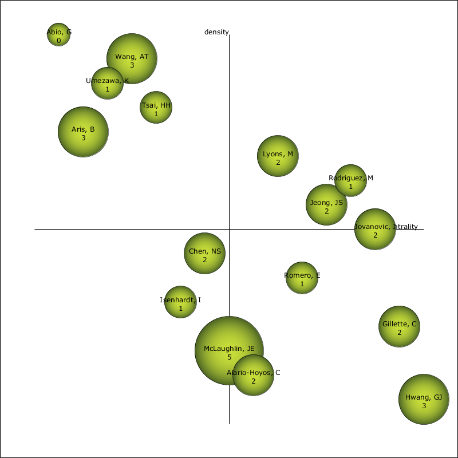
\includegraphics[width=\textwidth]{Fig06a.png}
 \subcaption{FLCL.}\label{fig06a}
 \end{minipage}
 \hfill
 \begin{minipage}{.45\textwidth}
 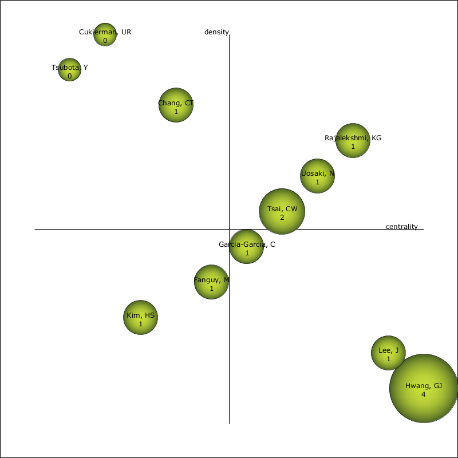
\includegraphics[width=\textwidth]{Fig06b.png}
 \subcaption{FLLE.}\label{fig06b}
 \end{minipage}
 \caption{Strategic diagram of authors of the entire production.}
 \label{fig06}
 \source{own elaboration.}
\end{figure}


\section{Discussion and Conclusions}\label{sec-discussion}
Both flipped learning and flipped classroom are newly created teaching methodologies that are gaining more prominence among teachers and researchers \cite{hinojo-lucena_incidence_2018}. Its pedagogical essence is based on the inversion of the moments of learning to combine the digital and face-to-face spaces \cite{lee_development_2017}, in such a way that the instructional process begins outside the conventional classroom \cite{borao_moreno_alisis_2016} when the students visualize the audiovisual content provided by the teacher \cite{el_miedany_flipped_2019,long_use_2017} and continues in the classroom itself promoting project-based learning, problem solving and –in short– enhancing the attractiveness of the learning process \cite{kostaris_investigating_2017}.

This research has focused on providing the scientific community with the terminological standardization necessary to guide their research to relevant topics in each of the fields studied. In addition, it will allow a prior and reflective analysis of the terminological choice (FLLE or FLCL) according to the research perspective to be proposed. The added value of the study is that there is currently no study that arises or analyzes the differences between the two terms, used in certain fields and in certain branches as synonyms, although the scientific community really makes differences in its research.

Although both the concept of flipped learning and that of flipped classroom are generally used as synonyms by teachers and researchers, the results obtained in this bibliometric study differ from this usual synonymic use due to certain different markers. 

The scientific output of FLCL is far superior to that of FLLE. For FLCL the type of document used by the scientists is communications, the main organization/institution is the University of North Carolina, the reference author is Keengwe, J., the source used is Advances in Social Science Education and Humanities Research and the authorship of the most cited article is \textcite{mclaughlin_flipped_2014}. On the other hand, in FLLE, the type of document used by the scientific community to show the results is the article, the main organization is the National Taiwan University of Science Technology, the reference author is Hwang, G.J., the source is INTED Proceedings and the most cited article is by \textcite{chen_is_2014}.

Despite these concomitants, both terms share Education Educational Research as the main area of publication, English as the most widely used language and the United States as the country of reference.

The themes of studies of both concepts vary from each other. While for FLCL the relevant concept –according to the bibliometric indicators– is "blended learning"; for FLLE the most predominant concepts are "university" and "flipped learning", although they maintain a common nexus between them, "flipped classroom", which appears to be relevant in both terms.

Differences are also observed if relevance is taken into account by periods, where FLCL shows a more settled line, centred on the "flipped classroom" theme, while for FLLE there is diversity between the different periods, being the "motivation" theme the only one that is repeated at least twice.

The marked connections between themes of the different periods offer a constant line, due to the marked terminological connections between the different concepts, but variants due to conceptual gaps and continuous terminological changes. In FLCL, "flipped classroom" is the concept that shows the greatest consistency and continuity over time; for FLLE, on the other hand, it is "flipped learning". Furthermore, in FLCL the conceptual connections established between themes are stronger than those marked in FLLE.

Moreover, it is pertinent to point out that the authors of greatest relevance in scientific production vary according to the field of study. While Lyons, M., Rodríguez, M. and Jeong, J.M. are for FLCL, Rajalekshmi, K.G., Uosaki, N., and Tsai, C.W. are for FLLE, not coinciding with the authors with greater production in their respective subjects. Likewise, the strategic diagrams allow us to glimpse that the authors with the greatest volume of production do not coincide with the most relevant authors for both FLCL and FLLE.

From the above, it can be concluded that FLCL and FLLE terminologies –despite being used by literature as synonyms or similar terminologies– in the scientific community are distinguished and differentiated, observing different trends and fields of study according to the concept used. In this fact lies –precisely– the prospective of the study, since it allows the scientific community to show the most appropriate fields of knowledge according to their line of research. In addition, it can be a starting point for seeking a terminological consensus that clearly delimits the field of terminology that encompasses each of the concepts analyzed.

Definitely, based on the prospect of this study, the results shown here are intended to solve an existing terminological problem in the scientific landscape. Consequently, it has been found that there are differences between the terms flipped classroom and flipped learning, so the educational community must keep both terms in mind and identify the specific connotations of each of them in order to present the results of their research. Therefore, it will allow the scientific community to know which are the main fields of research in each of the topics presented (FLLE and FLCL) and to know the main authors, the most productive countries and all the bibliometric factors related to each subject.

Among the limitations of the research is –on the one hand– the fact of compiling the diverse references and purifying the database in WoS and –on the other hand– the organizational reconstruction of the study at a temporal level, which led to new analyses and searches of the latest studies produced more immediately. Likewise, it should be noted that the results shown here have been approached from a general perspective and showing an intermediate level of specificity. Therefore, as a future line of research, it is proposed to expand the configuration of performance analysis to expand new connections and address other issues. Other notable options would be to carry out a study of a similar design, but using other relevant databases within the scientific field. In addition, it is proposed to investigate the existence of similar situations in which two concepts were applied under a synonym relationship to carry out their bibliometric study.

\printbibliography\label{sec-bib}

\end{document}
\end{tabularx}

